\begin{figure}[!hb]
    \centering
    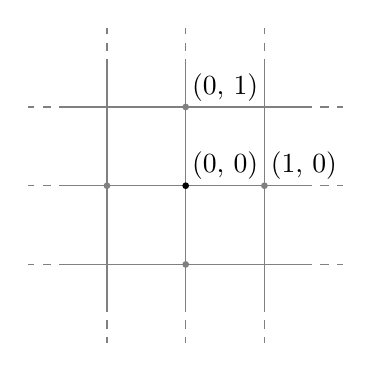
\begin{tikzpicture}
        \foreach \i in {-1, 0, 1} {
            \draw[gray] (-1.5, \i) -- (1.5, \i);
            \draw[gray] (\i, -1.5) -- (\i, 1.5);
            
            \draw[gray, dashed] (-1.5, \i) -- (-2.0, \i);
            \draw[gray, dashed] (\i, -1.5) -- (\i, -2.0);
            \draw[gray, dashed] (1.5, \i) -- (2.0, \i);
            \draw[gray, dashed] (\i, 1.5) -- (\i, 2.0);
        }
        \node at (0.5, 0.25) {(0, 0)};
        \node at (1.5, 0.25) {(1, 0)};
        \node at (0.5, 1.25) {(0, 1)};
        
        \filldraw (0, 0) circle (1pt);
        \filldraw[gray] (0, +1) circle (1pt);
        \filldraw[gray] (0, -1) circle (1pt);
        \filldraw[gray] (-1, 0) circle (1pt);
        \filldraw[gray] (+1, 0) circle (1pt);
    \end{tikzpicture}
    \caption{The origin (black) and its 4 neighbours (grey) on the square lattice}
    \label{fig:square_lattice}
\end{figure}